\documentclass[11pt]{article}
    \title{\textbf{Computer Architecture}\\[0.5em]
    \large Project Step 2: Arithmetic Logic Unit}
    
    \author{Group ``Orange": Chloe MacGregor, Nathaniel Jefferson, Rex Almerico}
    \date{March 30, 2026}

    \addtolength{\topmargin}{-3cm}
    \addtolength{\textheight}{3cm}

\usepackage{listings}
\usepackage{color}

\usepackage{graphicx}
\graphicspath{ {../images/} }

\definecolor{dkgreen}{rgb}{0,0.6,0}
\definecolor{gray}{rgb}{0.5,0.5,0.5}
\definecolor{mauve}{rgb}{0.58,0,0.82}

\lstset{frame=tb,
  language=Java,
  aboveskip=3mm,
  belowskip=3mm,
  showstringspaces=false,
  columns=flexible,
  basicstyle={\small\ttfamily},
  numbers=none,
  numberstyle=\tiny\color{gray},
  keywordstyle=\color{blue},
  commentstyle=\color{dkgreen},
  stringstyle=\color{mauve},
  breaklines=true,
  breakatwhitespace=true,
  tabsize=3
}

\begin{document}

\maketitle
\thispagestyle{empty}

\section{Objectives}
The goal of this step in the project is to create the full 4 bit ALU functions (And, Nand, Or, Nor, Xor, Xnor, Not, 2x4-bit input / 2x4-bit output Arithmetic Shifter, Addition, Subtraction, Multiplication, and Division), using the building blocks of the 1 bit logic circuits.


\section{One-bit Arithmetic}
Computers understand mathematics in terms of finite binary digits (bits), so building arithmetic circuits requires starting with single bit arithmetic.
\subsection{Verilog Code}
\lstinputlisting[breaklines]{../step-1/code.v}

\pagebreak
\subsection{1-Bit Circuit Unit Tests}
We separated each unit tests into its own testbench files that correspond each to their own code module. Below is the test for the not circuit:
\lstinputlisting[breaklines]{../step-1/tests/test_not.v}
   
and the corresponding output waveforms\\
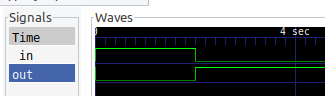
\includegraphics{not_waveform}

\pagebreak
and for the nand circuit:
\lstinputlisting[breaklines]{../step-1/tests/test_nand.v}
   
and the corresponding output waveforms\\
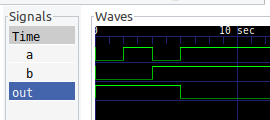
\includegraphics{nand_waveform}

\pagebreak
and for the nor circuit:
\lstinputlisting[breaklines]{../step-1/tests/test_nor.v}
   
and the corresponding output waveforms\\
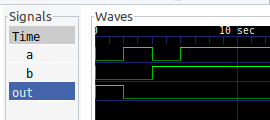
\includegraphics{nor_waveform}

\pagebreak
and for the shift circuit:
\lstinputlisting[breaklines]{../step-1/tests/test_shift.v}
\pagebreak
and the corresponding output waveforms\\
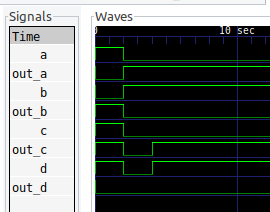
\includegraphics{shift_waveform}



\section{Four-bit Logic}
We designed the following circuits using Verilog:
\subsection{AND, NAND, OR, NOR, XOR, XNOR, NOT, and Shift}
\lstinputlisting[language=Verilog]{code/logic/and4.v}
\lstinputlisting[language=Verilog]{code/logic/nand4.v}
\pagebreak
\lstinputlisting[language=Verilog]{code/logic/or4.v}
\lstinputlisting[language=Verilog]{code/logic/nor4.v}
\lstinputlisting[language=Verilog]{code/logic/xor4.v}
\lstinputlisting[language=Verilog]{code/logic/xnor4.v}
\lstinputlisting[language=Verilog]{code/logic/not4.v}
\lstinputlisting[language=Verilog]{code/logic/shifter4.v}

\section{Four-bit Arithmetic}
We designed the following circuits using Verilog:
\subsection{ADD, SUB, MUL, DIV}
\lstinputlisting[language=Verilog]{code/arithmetic/adder4.v}
\lstinputlisting[language=Verilog]{code/arithmetic/subtractor4.v}
\pagebreak
\lstinputlisting[language=Verilog]{code/arithmetic/multiplier4.v}
\lstinputlisting[language=Verilog]{code/arithmetic/divider4.v}

\pagebreak

\section{Circuit Unit Tests For Logic}

%there are lots of comments in this section because gtkwave looks weird for me
%once all the pictures are taken and aptly named all comments after this can be uncommented

We separated each of the unit tests into their own testbench files that each correspond to their own code module. Below is the test for the 4-bit AND circuit:
\lstinputlisting[language=Verilog]{tests/test_and4.v}
\pagebreak
and the corresponding output waveform\\
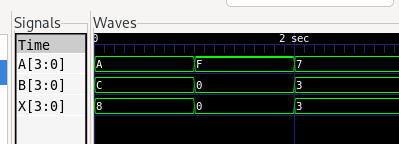
\includegraphics{and4_waveform.png}
\pagebreak

NAND circuit:
\lstinputlisting[language=Verilog]{tests/test_nand4.v}
\pagebreak
and the corresponding output waveform\\
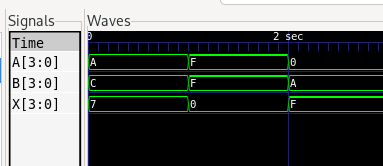
\includegraphics{nand4_waveform.png}
\pagebreak

OR circuit:
\lstinputlisting[language=Verilog]{tests/test_or4.v}
\pagebreak
and the corresponding output waveform\\
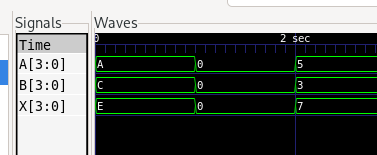
\includegraphics{or4_waveform.png}
\pagebreak

NOR circuit:
\lstinputlisting[language=Verilog]{tests/test_nor4.v}
\pagebreak
and the corresponding output waveform\\
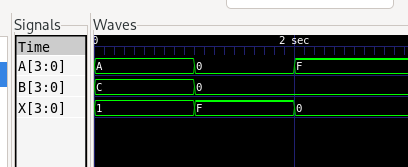
\includegraphics{nor4_waveform.png}
\pagebreak

XOR circuit:
\lstinputlisting[language=Verilog]{tests/test_xor4.v}
\pagebreak
and the corresponding output waveform\\
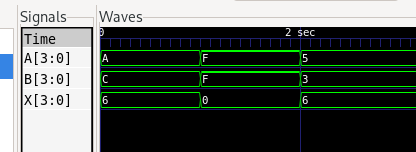
\includegraphics{xor4_waveform.png}
\pagebreak

XNOR circuit:
\lstinputlisting[language=Verilog]{tests/test_xnor4.v}
\pagebreak
and the corresponding output waveform\\
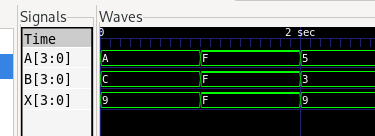
\includegraphics{xnor4_waveform.png}
\pagebreak

NOT circuit:
\lstinputlisting[language=Verilog]{tests/test_not4.v}
\pagebreak
and the corresponding output waveform\\
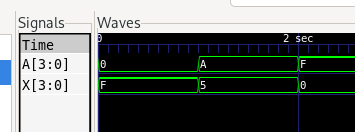
\includegraphics{not4_waveform.png}
\pagebreak

Shift circuit:
\lstinputlisting[language=Verilog]{tests/test_shifter4.v}
\pagebreak
and the corresponding output waveform\\
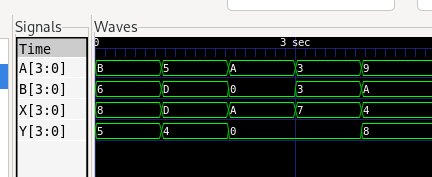
\includegraphics{shifter4_waveform.png}
\pagebreak

\subsection{Circuit Unit Tests for Arithmetic}

ADD circuit:
\lstinputlisting[language=Verilog]{tests/test_adder4.v}
\pagebreak
and the corresponding output waveform\\
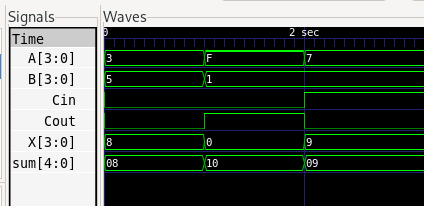
\includegraphics{adder4_waveform.png}
\pagebreak

SUB circuit:
\lstinputlisting[language=Verilog]{tests/test_subtractor4.v}
\pagebreak
and the corresponding output waveform\\
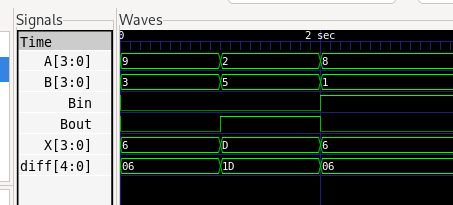
\includegraphics{subtractor4_waveform.png}
\pagebreak

MUL circuit:
\lstinputlisting[language=Verilog]{tests/test_multiplier4.v}
\pagebreak
and the corresponding output waveform\\
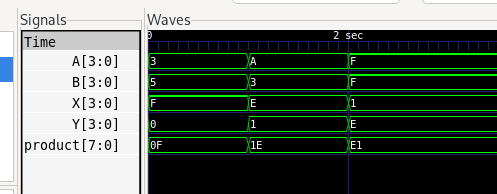
\includegraphics{multiplier4_waveform.png}
\pagebreak

DIV circuit:
\lstinputlisting[language=Verilog]{tests/test_divider4.v}
\pagebreak
and the corresponding output waveform\\
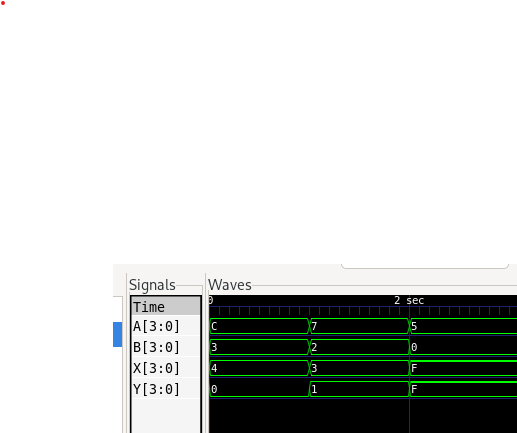
\includegraphics{divider4_waveform.png}
\pagebreak

\section{Conclusion}
In this step of the project, we successfully designed and tested the 4-bit ALU functions using Verilog. We created separate modules for each logic and arithmetic function, and we verified their correctness through unit tests and waveform analysis. This lays a solid foundation for integrating these components into a complete ALU in the next step of the project.

\end{document}
